
\section{Approfondimenti sul BUS IEEE 488 - GPIB}
Presenta 5 linee di GIM tra le quali
\begin{itemize}
 \item IFC
 \item REN
 \item ATN
 \item SRQ
 \item EOI
\end{itemize}
tre linee per la sincronizzazione che seguono il protocollo ``handshake'',
8 linnee per la trasmissione dati e 8 linee di riferimento (GND).

Un esempio di processo di misura da automatizzare è ancora il collaudo di un
doppio bipolo che realizza un filtro passa basso, il banco è costituito da tre
strumenti e un controller.
Il controller è un PC con interfaccia IEEE488, un counter a due canali, una
sorgente a singolo canale e un multimetro digitale a due canali.
Anche gli strumenti, come il PC sono dotati di interfaccia.

Il counter serve a misurare lo sfasamento tra i segnali isofrequenziali, il
multimetro misura il guadagno introdotto dal filtro, solitamente un guadagno
unitario nella banda passante che si riduce man mano entrando nella frequenza
di transizione, oltre la frequenza di taglio.

Il controller attesta la linea IFC e subito dopo da un secondo comando
universale unilinea REN in cui specifica alle unià periferiche che riceveranno
i comandi tramite interfaccia e non tramite pannello. Si attesta poi la linea
ATN e la stazione di misura viene posta in regime ``command mode''.

Il controller in questo funzionamento assegna dei ruoli agli strumenti mediante
un meccanismo di indirizzamento, ad ogni strumento sarà assegnato un indirizzo,
un intero che va da 1 a 30, per specificare quest'indirizzo si utilizzano 5 bit.

Con 5 bit si realizzerebbero $2^5$ combinazioni ma l'indirizzo 0 è riservato al
controller mentre l'indirizzo 31 è necessario all'abilitazione di un indirizzo
secondario, come ad esempio un modulo particolare di un certo strumento.

Sono comunque poche le applicazioni che necessitano del meccanismo di
indirizzamento secondario.

Si assegni alla sorgente l'indirizzo 1, al multimetro l'indirizzo 2 e al
counter l'indirizzo 8.
Per configurare inizialmente la sorgente va inviato un comando in regime
``device mode'' comprensibile solo alla sorgente, dopo averle assegnato un
ruolo, si riserva il bus ad una comunicazione dedicata tra un talker e un
listener.

Per assegnare il ruolo di listener alla sorgente si utilizzano lel linee dati
usando i 5 bit meno significativi l'indirizzo dello strumento, assegnando un
ruolo mediante il sesto e il settimo bit, l'ottavo bit rispetta la regola della
parità.

Il controller assegna il ruolo di listener al dispositivo con indirizzo 1

\verb|00100001 - A - !|

Si configura il controller come listener

\verb|11000000 - \@ - MTA0|

Si rilascia infine la linea attention (ATN) passando al regime device mode, il
counter e il multimetro non hanno visto il loro indirizzo, restando in idle.

La comunicazione sul BUS prevede sempre un solo talker ma può avere più
listener a patto che comprendano lo stesso linguaggio.

Gli strumenti di misura hanno sempre in allegato dei manuali, o una
documentazione con una sezione riservata alla programmazione dello strumento.

Un comando che solitamente si usa per configurare la sorgente è il comando

\verb|APPLy:SINusoidal 10,1000,0|

Nella sintassi estesa si può aggiungere l'unità di misura dei valori.
La sintassi contratta è composta solo dalle parti in maiuscolo, la sintassi è
decisa dal costruttore.
Si potrebbe in teoria assegnare un comando per ciascun carattere, riducendo il
numero di caratteri da inviare.

La velocità di throughput può raggiungere velocità pari al megabyte/s.
Lo standard richiede di non utilizzare cavi di lunghezza maggiori.

Rendere il linguaggio dello strumento stringato si è riscontrato che i comandi
per attivare le funzioni sono più semplici da memorizzare.
La scelta dei costruttori è stata quella di configurare i comandi da renderli
facilmente memorizzabili.

Durante la configurazione, la sorgente inizia a a generare il segnale stabile,
rendendo l'interfaccia indipendente.

All'invio di ogni byte in device mode, si attiva una procedura di
configurazione per lo scambio dei dati con conseguente sincronizzazione

Se lo strumento riceve un comando errato, va in errore.

Il talker configura le linee dati utilizzando la procedura di handshake per
sincronizzare la comunicazione, quando ha terminato il messaggio, invia l'EOI,
End Of Identify

Terminata la comunicazione dal sistema sorgente, a talker torna il possesso del
bus.

In regime command mode il controller associa il ruolo di listener
all'indirizzo 2

\verb|00100010|

e ancora il ruolo di listener a sé stesso, vanno ora inviati dei comandi di
\textit{deselezione} degli strumenti precedentemente attivati, ad esempio si
invia il seguente comando per deselezionare i listener precedentemente attivati

\verb|00111111 - ?|

oppure per deselezionare i talker con il carattere ``\_''

\verb|01011111 - _|

Per ottenere il risultato dal multimetro dopo averlo impostato come listener si
invia un comando di QUERY, terminato da punto interrogativo (?)

\verb|MEAS:CH1:VAC?|

Lo strumento deve conservare il risultato perché dopo una QUERY allo strumento
verrà assegnato il ruolo di parlatore e invierà il risultato al listener, il
ruolo di parlatore al dispositivo 2 si invia con il carattere B, ancora una
volta il controller si imposta come listener con il carattere ``barra
spaziatrice''

\verb|01000010 - B|

\verb|10100000 - " "|

Quando il multimetro termina la comunicazione si ritorna in regime di command
mode, si ripete la procedura per rieseguire la misura sul canale 2 (\verb|CH2|).

Lo stesso processo si ripete per il counter per eseguire la misura di
sfasamento, deseleziona precedenti listener e talker, invia una QUERY al
counter dopo averlo impostato come listener, dopo si imposta come talker per
permettergli l'invio del risultato.



Quelli presentati sono comandi multi linea universali, perché utilizzano più
linee per comunicare con i dispositivi, possono essere specifici se hanno un
indirizzo specifico e si riferiscono ad un singolo dispositivo oppure possono
essere aspecifici se inviano un comando a tutti i dispositivi come la
deselezione.

Nei linguaggi di programmazione moderni tutti questi comandi sono contenuti in
librerie che eseguono lettura e scrittura di dati da e verso il BUS mediante
comandi più semplici come ``\textit{bus read}'' e ``\textit{bus write}''.

\subsection{Driver delle linee}
Per attestare o rilasciare una linea si utilizza un transistor bipolare, è un
dispositivo comandato in corrente, iniettando una corrente di base $i_B$ si ha
la conduzione, altrimenti senza alcuna corrente si pone in regione di
interdizione, nel driver si collega il transistor mediante una resistenza di
``pull-up``, la linea va in contatto elettrico con il morsetto collettore del
BJT.

Si riporta la caratteristica del transistor, una famiglia di curve in funzione
della corrente di base $I_B$
\begin{figure}[h]
\centering
\includegraphics[width=0.5\linewidth]{BJT}
\caption{Carattaristica di un BJT}
\end{figure}

Abbondando con la corrente di base si manda in saturazione il BJT e si attesta
la linea, ponendo $V_{CE} = 0$, eliminando la corrente di base invece la
$V_{CE}$ può essere piccola o grande, questo fa sì che se la linea è condivisa
tra più driver potrebbe accadere che se un transistor vuole la linea attestata
e un altro transistor la vuole rilasciata prevarrà il driver che attesta la
linea, la corrente nel transistor in saturazione aumenta, provenendo anche
dall'alimentazione del driver interdetto; per questo motivo si utilizza il
potenziale basso per il valore logico 1, se c'è una sola interfaccia che vuole
attestare la linea, quella linea si attesta.
È implementata la logica wired-OR, basta almeno un valore 1 affinché tutta la
linea sia 1.

\begin{figure}[h]
\centering
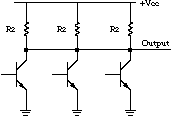
\includegraphics[width=0.5\linewidth]{wired-or}
\caption{Wired OR}
\end{figure}

Esiste un problema detto di fan-in se in un sistema con più periferiche un solo
driver assorbe correnti dagli altri driver diventerebbe troppo elevata, per
questo motivo lo standard impone un numero massimo di dispositivi pari a 15,
per non sovraccaricare il transistor in saturazione.


Non tutte le linee sono condivise, gli strumenti di misura ad esempio non
possono pilotare le linee IFC, REN e ATN riservate al controller, possono solo
osservarne lo stato ma non alterarlo.

\subsection{Sincronizzazione}
Il clock dei diversi hardware e strumenti non è standardizzato, ciascun
dispositivo avrà il suo clock, sono definiti moduli ''asincroni`` tra loro.
Sistemi con moduli sincroni sono invece solitamente ospitati su una stessa
scheda; in una stazione automatica di misura si utilizzano strumenti
stand-alone, intercambiabili e utilizzabili in situazioni diversi.
Alcuni sistemi VXI, PCI gli strumenti stanno su scheda invece e vanno collocati
in un'altra scheda, utilizzando il clock del dispositivo ''ospite``.

Affinchè la comunicazione avvenga correttamente tra moduli asincroni va gestita
la sincronizzazione, le linee utilizzate a tale scopo sono 3, riferite con i
seguenti acronimi
\begin{itemize}
 \item DAV: ''Data Valid`` oppure ''Data Available``, gestita da chi invia il
dato
 \item NRFD: Not Ready For Data gestita da chi riceve i dati, non sono pronto a
ricevere i dati
 \item NDAC: Not Data ACcepted, gestita da chi riceve i dati, non ho ricevuto i
dati
\end{itemize}

Chi deve parlare configura le linee dati DIO in un certo istante con un
carattere arbitrario da trasferire, comunica che i dati sono pronti dopo averli
configurati, dopo essersi accertato che le periferiche sono pronte per ricevere
il dato e se hanno acquisito il dato precedente.

La linea NRFD è condivisa tra più ascoltatori, di conseguenza per quanto
precedentemente esposto, quando TUTTI gli strumenti rilasciano la linea, anche
il più lento, la linea viene rilasciata; solo allora la periferica più veloce
attesta nuovamente la linea nell'attesa della ricezione dei dati. Dopo che i
dati sono stati dichiarati validi, via via che tutte le periferiche verificano
e accettano i dati, rilasciano la linea NDAC, quando anche la periferica più
lenta rilascia la linea NDAC la linea viene rilasciata, solo allora il
parlatore, che intanto osserva la linea NDAC, riconfigura la linea dati
inserendo il dato successivo, il ciclo si ripete.

\begin{figure}[h]
\centering
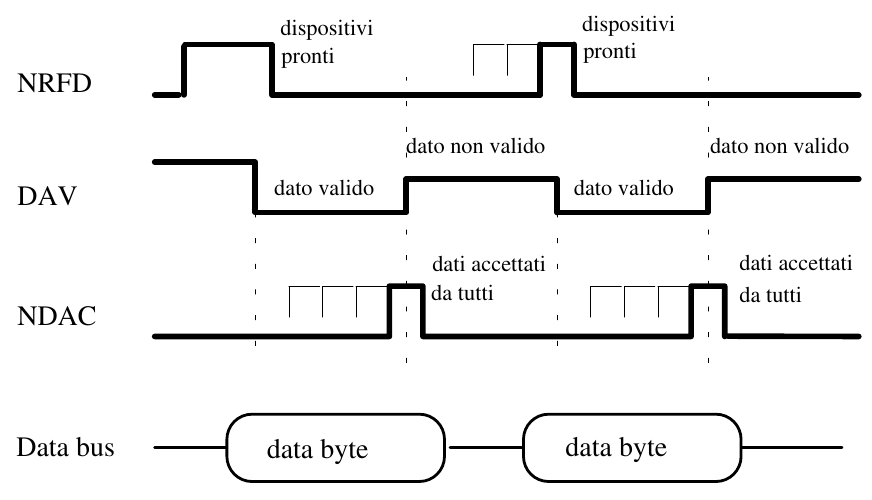
\includegraphics[width=0.7\linewidth]{sincronizzazione}
\end{figure}
Il meccanismo wired-OR permette di mantenere il dato sul BUS finché anche la
periferica più lenta non lo ha interamente acquisito, si evitano le letture
multiple alle periferiche veloci e si permette alle periferiche lente di
acquisire interamente i dati.


\subsection{Gestione delle richieste di servizio SRQ}
Quando uno strumento riceve una QUERY, mentre esegue la sua elaborazione il BUS
non resta occupato, quando ha terminato le misurazioni attesta la linea SRQ,
non si può sapere quale strumento abbia attestato la SRQ, va eseguita una
procedura di polling, di interrogazione. Esistono due tipologie di polling,
seriale e parallelo, il polling seriale consiste nell'interrogazione di tutti
gli strumenti in serie, uno alla volta.

C'è un comando multilinea universale che corrisponde al carattere ASCII SPE,
''Serial Poll Enable'' tutti gli strumenti capiscono che se sono chiamati ad
essere talker sul BUS devono trasferire sul BUS il contenuto dello status byte,
se il settimo bit è alto allora indica che quello strumento ha precedentemente
effettuato la richiesta SRQ, i restanti bit contengono l'informazione sul
motivo della richiesta.

Il polling seriale deve essere esaustivo, non posso sapere quanti strumenti
abbiano attestato la linea SRQ, terminato il polling si invia la richiesta SPD
``Serial Poll Disable'' al fine di rilasciare la linea SRQ.

La procedura di polling parallelo invece è più efficiente anche se richiede una
procedura di configurazione iniziale più onerosa, si dà un comando detto PPC
``Parallel Poll Configure'' ovvero avvia una procedura di configurazione al
parallel poll, ad ogni strumento viene assegnata una linea dati da
attestare (sono presenti 8 linee dati), una volta ricevuta la SRQ si può sapere
in anticipo quale strumento l'abbia richiesta leggendo quale linee dati sono
state attestate, in command mode(ATN) l'attestazione della linea EOI invia una
richiesta di identificazione, se la periferica aveva effettuato una richiesta
di servizio agisce direttamente sulla linea dati ponendo alto il bit che le era
stato assegnato.

Se il numero di dispositivi è maggiore di 8 si possono assegnare più
dispositivi alla stessa linea, ripetendo la procedura di polling seriale su un
gruppo più piccolo di dispositivi.

Terminata la configurazione di parallel poll si invia il comando PPU ``Parallel
Poll Unconfigure`` per disabilitare la risposta di tutti i dispositivi al
parallel poll.

